\documentclass[10pt,a4paper]{article}
\usepackage{amsmath}
\usepackage{amssymb}
\usepackage{graphicx}
\usepackage{color}
\usepackage{fancyhdr}
\usepackage{fancyvrb}
\usepackage[margin=3.5cm]{geometry}
\usepackage{framed}
\usepackage{enumerate}
\usepackage{textcomp}
\def\ket#1{\left|#1\right\rangle}
\def\bra#1{\left\langle#1\right|}
\def\braket#1{\left\langle#1\right\rangle}

\definecolor{linkcol}{rgb}{0.0, 0.0, 0.5}
\usepackage[colorlinks=true,urlcolor=linkcol,citecolor=black,linkcolor=linkcol]{hyperref}

\renewcommand\thesection{0.\arabic{section}}
\renewcommand\thesubsection{\thesection.\arabic{subsection}}

\fancyhf{}
\lhead{\tiny Y.~D.~Chong (2016)}
\rhead{\scriptsize MH2801: Complex Methods for the Sciences}
\lfoot{}
\rfoot{\thepage}
\pagestyle{fancy}

\makeatletter
\def\PY@reset{\let\PY@it=\relax \let\PY@bf=\relax%
    \let\PY@ul=\relax \let\PY@tc=\relax%
    \let\PY@bc=\relax \let\PY@ff=\relax}
\def\PY@tok#1{\csname PY@tok@#1\endcsname}
\def\PY@toks#1+{\ifx\relax#1\empty\else%
    \PY@tok{#1}\expandafter\PY@toks\fi}
\def\PY@do#1{\PY@bc{\PY@tc{\PY@ul
\def\PYZdl{\char`\$}
\def\PYZhy{\char`\-}
\def\PYZsq{\char`\'}
\def\PYZdq{\char`\"}
\def\PYZti{\char`\~}

\begin{document}

\noindent
\underline{\textbf{\LARGE 0. Mathematical Functions}}
\vskip 0.1in

This is a course on complex methods in the physical sciences. Before
dealing with complex numbers, however, let us undertake a brief review
of real mathematical functions and their properties.

\section{Real functions}\label{real-functions}

A mathematical function, denoted $f$, takes an input $x$ (which is
also called an \textbf{argument}), and returns an output $f(x)$. For
now, we consider the case where both $x$ and $f(x)$ are real
numbers. The set of possible inputs is called the \textbf{domain} of the
function, and the set of possible outputs is called the \textbf{range}.

A well-defined function must have an unambiguous output: for any $x$
in the domain, $f(x)$ must be a specific number in the range. In other
words, functions must be either one-to-one (injective) mappings, or
many-to-one mappings. They can't be one-to-many or many-to-many. This is
illustrated by the following graphs:

\begin{figure}[h]
  \centering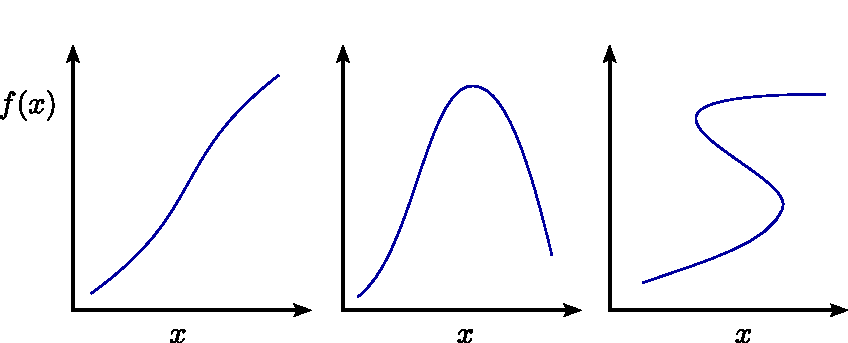
\includegraphics[width=0.7\textwidth]{mathfunctions}
\end{figure}

\noindent
Simple examples of mathematical functions are those based on elementary
algebra operations:
\begin{align*}
  f(x) &= x + 2 \,\;\;\qquad\qquad \text{(a one-to-one function)} \\
  f(x) &= x^2 + 2x + 4 \qquad \text{(a many-to-one function)}
\end{align*}

\subsection{Exponential and logarithm}
\label{Exponentials}

The exponential function $\exp(x)$ is a particularly important and
ubiquitous function. You've probably come across this function before,
but let's remind ourselves of how and why it's defined. We begin with a
meditation on what it means to take a number $x$ to the power of
$y$:
\begin{equation}
  f(x) = x^y.
\end{equation}

For values of $y$ in natural numbers $\mathbb{N} \equiv
\{1,2,3,\dots\}$, the power operation simply means multiplying $x$ by
itself $y$ times. For example, $x^4 = x \cdot x \cdot x \cdot x$. But
what about non natural number powers, like $x^{-1}$ or $x^{1/2}$ or
$x^{3.14}$? To answer this, we introduce the natural exponential
function, defined as the following limiting infinite series:
\begin{equation}
  \exp(x) \equiv \lim_{n\rightarrow\infty} \left(1+\frac{x}{n}\right)^n = 1 + \sum_{n=1}^\infty\frac{x^n}{n!}, \qquad x \in \mathbb{R}.
\end{equation}

It is left as an exercise for you to show that the two infinite series
formulas in this definition are equivalent.  Note that both the
infinite series use natural number powers only. The function's domain
is the entire set of real numbers, $\mathbb{R}$, and its range is the
set of positive numbers, $\mathbb{R}^+$. Its graph is as follows:

\begin{figure}[h]
  \centering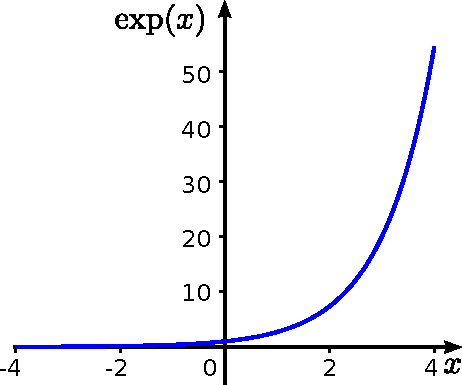
\includegraphics[width=0.4\textwidth]{exponential}
\end{figure}
    
A highly noteworthy feature of $\exp(x)$ is that, for $x > 0$, it
becomes large extremely quickly with increasing $x$. For $x < 0$, it
becomes small extremely quickly with decreasing $x$. It also has a
number of other useful mathematical properties. For instance, one can
show that
\begin{equation}
  \exp(x+y) = \exp(x)\,\exp(y) \quad \forall x, y \in \mathbb{R}.
\end{equation}
(Try proving this as an exercise.)  As a corollary,
\begin{equation}
  \exp(-x) = 1/\exp(x).
\end{equation}
Because the exponential function is one-to-one, its inverse is also a
well-defined function. We call this the natural logarithm:
\begin{equation}
\ln(x) \equiv y \;\; \mathrm{such}\;\mathrm{that}\;\;\exp(y) = x.
\end{equation}
Unless otherwise noted, we will always mean the natural logarithm when
we say ``logarithm''. The domain of the logarithm is $y \in
\mathbb{R}^+$, and its range is $\mathbb{R}$.  Its graph is shown
below:

\begin{figure}[h]
  \centering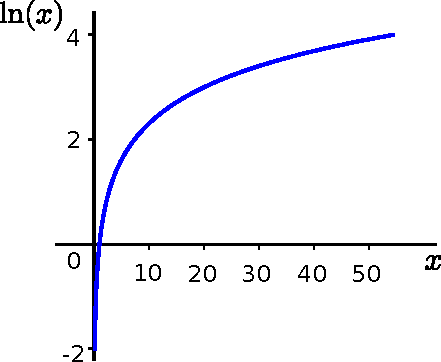
\includegraphics[width=0.4\textwidth]{logarithm}
\end{figure}
Observe that for $x>0$, $\ln(x)$ increases very slowly with $x$.  This
is the opposite of the exponential function's behavior, where
$\exp(x)$ increases very quickly with $x$. One can also show that the
logarithm satisfies the important property
\begin{equation}
\ln(xy) = \ln(x) + \ln(y).
\end{equation}
Hence, the power operation interacts with the exponential and
logarithm functions in the following manner:
\begin{align}
  \ln(x^y) &= y \ln(x)\qquad\quad&\mathrm{for}&\;\;y \in \mathbb{N} \\
  \Rightarrow\quad\quad x^y &= \exp[y \ln(x)] \quad &\mathrm{for}&\;\;y \in \mathbb{N}.
\end{align}

Now we have the tools we need to discuss the issue raised at the
beginning of this section, i.e.~how to deal with the concept of a
non-natural power. Let us generalize the above equation by assuming that
it continues to hold true for any positive $x$ and real $y$, not
just for $y \in \mathbb{N}$. In other words, we treat this as our
\emph{definition} of what it means to perform the power operation, for
non-natural powers:
\begin{equation}
  x^y \equiv \exp[y \ln(x)] \qquad\; \mathrm{for}\; x \in \mathbb{R}^+, \;y \notin \mathbb{N}.
  \label{powerdef}
\end{equation}
Based on this definition, the power operation always gives a positive
result. You can also check for yourself that, for $y \in \mathbb{N}$,
the formula is consistent with the results based on using the standard
definition of ``multiply $x$ by itself $y$ times''.

This generalization of the power operation leads to many extremely
important consequences:
\begin{itemize}
\item 
  Raising a positive number to the zeroth power gives unity:
  $\displaystyle x^0 = 1$.
\item
  Negative powers are reciprocals:
  \begin{equation*}
    x^{-y} =
    \exp[-y\ln(x)] = \exp[-\ln(x^y)] = \frac{1}{x^y}.
  \end{equation*}

\item
  The exponential function can itself can be written as a power:
  \begin{equation*}
    \exp(y) = e^y,
  \end{equation*}
  where $e \equiv \exp(1) = 2.718281828459\dots$
\item
  Non-integer powers are only defined for non-negative $x$, since the
  logarithm in the definition does not accept negative inputs.
\end{itemize}

\subsection{Trigonometric functions}
\label{trigo}

The fundamental trignonometric functions $\sin(\theta)$,
$\cos(\theta)$, and $\tan(\theta)$ can be defined in terms of the
geometric ratios of the sides of right-angled triangles, as shown here:

\begin{figure}[h]
  \centering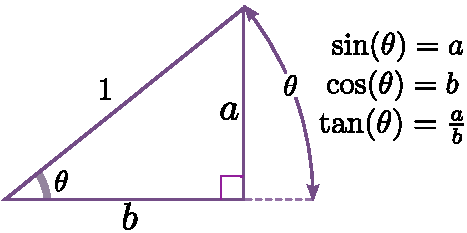
\includegraphics[width=0.4\textwidth]{trigonometry}
\end{figure}

In this basic definition, the domain is $\theta \in [0, \,\pi/2)$,
  where the angle $\theta$ is given in radians. We can generalize the
  definitions to allow for negative values of $a$ and/or $b$, using
  the following scheme:

\begin{figure}[h]
  \centering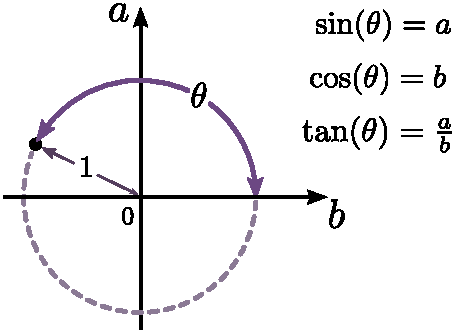
\includegraphics[width=0.4\textwidth]{trigonometry2}
\end{figure}

\noindent
Now the angle $\theta$ lies within a larger domain: $\theta \in
[0,\,2\pi)$.

We can further generalize the trigonometric functions by extending the
domain to all real numbers: $\theta \in \mathbb{R}$. This is done by
treating all values of $\theta$ modulo $2\pi$ as equivalent,
i.e.~$f(\theta + 2\pi) = f(\theta)$. With this generalization, the
trigonometric functions become many-to-one functions.


From the
\href{http://en.wikipedia.org/wiki/Pythagoras_theorem}{Pythagorean
  theorem},
\begin{equation}
\big[\sin(\theta)\big]^2 + \big[\cos(\theta)\big]^2 = 1.
\end{equation}
Armed with this result, we can go on to prove a variety of identities,
like the addition identities
\begin{align}
  \begin{aligned}
    \sin(\theta_1 + \theta_2) &= \sin(\theta_1) \cos(\theta_2) + \cos(\theta_1)\sin(\theta_2) \\\cos(\theta_1 + \theta_2) &= \cos(\theta_1) \cos(\theta_2) - \sin(\theta_1)\sin(\theta_2)\end{aligned}
\end{align}
As you may recall, these identities can be proved by trigonometry; the
proofs involve drawing the correct set of triangles, and choosing
which sides of the triangles to put into the Pythagorean formula.  (As
an exercise, try proving either of the above identities
trigonometrically.) There are two problems with such proofs: (i) they
require a certain amount of ingenuity in choosing which triangle
diagrams to draw, and (ii) it's not immediately obvious that the
proofs work if the angles lie outside $[0,\pi/2]$. Happily, there is a
solution to both problems: as we'll soon see, trigonometric identities
of this sort can be proven algebraically, with the aid of complex
numbers.

\subsection{Hyperbolic functions}\label{hyperbolic-functions}

The hyperbolic functions are important special functions which are
defined in terms of exponentials:
\begin{align}
\begin{aligned}\sinh(x) &= \frac{1}{2}\left(e^{x} - e^{-x}\right) \\ \cosh(x) &= \frac{1}{2}\left(e^{x} + e^{-x}\right) \\ \tanh(x) &= \frac{e^{x} - e^{-x}}{e^{x} + e^{-x}}\end{aligned}
\end{align}
These functions have properties intriguingly similar to the trignometric
functions. For example, they have addition identities
\begin{align}
  \begin{aligned}\sinh(x+y) &= \sinh(x)\cosh(y) + \cosh(x)\sinh(y) \\
\cosh(x+y) &= \cosh(x)\cosh(y) + \sinh(x)\sinh(y)\end{aligned}
\end{align}
Because of these identities, it's sometimes more convenient to work with
hyperbolic functions rather than exponentials. We'll deal with such
situations when we get to them.

\section{Continuity}

\textbf{Continuity} is an important concept which refers to the idea
that a function's output $x$ does not make any abrupt jumps as we vary
the input $x$. A function can be continuous over its entire domain, or
only a subset of its domain (mathematicians have even come up with
functions that are discontinuous everywhere in their domain, but such
pathological cases are uncommon in physics applications). For example,
$f(x) = 1/x$ is discontinuous at the origin $x = 0$. So is the step
function
\begin{equation}
\Theta(x) = \left\{\begin{array}{ll} 1, &\;\;\;\textrm{for} \; x \ge 0\\ 0,&\;\;\; \textrm{otherwise.}\end{array}\right.
\end{equation}

The rigorous definition of continuity is as follows. A function is
continuous at a point $x_0$ if, for any $\epsilon > 0$, we can find
a $\delta > 0$ such that setting $x$ closer to $x_0$ than a
distance of $\delta$ brings $f(x)$ closer to $f(x_0)$ than the
specified distance $\epsilon$.

This sounds like a very complicated sentence (and it is!), and it may
be easier to understand it using the illustration below:

\begin{figure}[h]
  \centering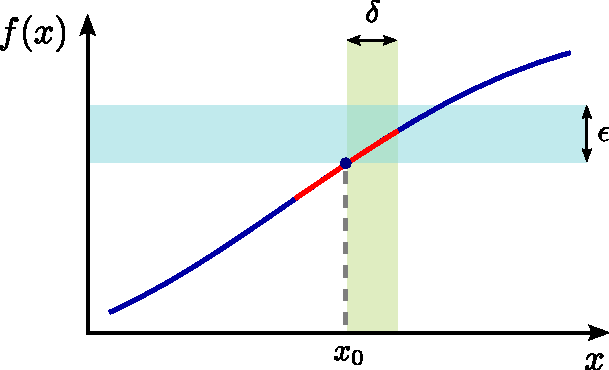
\includegraphics[width=0.5\textwidth]{continuity}
\end{figure}

\noindent    
Here is counter-example, showing a function with a discontinuity at
some $x_0$:

\begin{figure}[h]
  \centering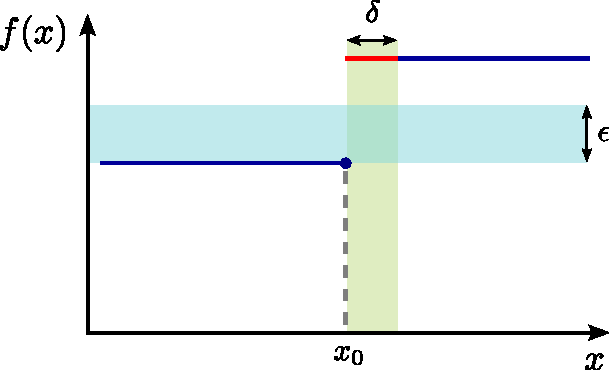
\includegraphics[width=0.5\textwidth]{discontinuity}
\end{figure}

\noindent
If we choose $\epsilon$ smaller than the gap, then no matter what
value of $\delta > 0$ we try, any choice of $0 < x < \delta$ gives a
value of $f(x)$ that's further than $\epsilon$ from $f(x_0)$. Hence,
the continuity condition is violated for sufficiently small choices of
$\epsilon = 1/2$, and we say that $f(x)$ is \textbf{discontinuous} at
$x_0$.

\section{Exercises}\label{exercises}

\begin{enumerate}
\item 
  Prove that the two infinite series definitions of the exponential
  are equivalent:
  \begin{equation*}
    \lim_{n\rightarrow\infty} \left(1+\frac{x}{n}\right)^n = 1 +
    \sum_{n=1}^\infty\frac{x^n}{n!}.
  \end{equation*}

\item
  Prove that $\exp(x+y) = \exp(x)\,\exp(y)$, using the
  definition
  \begin{equation*}
    \exp(x) \equiv 1 + \sum_{n=1}^\infty\frac{x^n}{n!}.    
  \end{equation*}
  In this proof, avoid using the concept of ``raising to the power''
  of a non-natural number (this is so that we can use this property of
  the exponential function in \hyperref[powerdef]{the definition of a
    non-natural number power}).

\item
  One of the most important features of the exponential function
  $\exp(x)$ is that it becomes large \textit{extremely} quickly with
  increasing $x$. To illustrate this behavior, consider the graph of
  the exponential function in Section \ref{Exponentials}. The graph
  plots up to $x = 4$, and the height of the graph on the page should
  be around 4cm. Suppose we keep the same resolution, and plot up to
  $x = 10$; how high would the graph be?  What about if we plotted up
  to $x = 20$?

\item
  Prove, using the \hyperref[powerdef]{generalized definition of the
    power operation}, that
  \begin{equation*}
    \exp(x) = [\exp(1)]^x.
  \end{equation*}

\item
  A ``non-natural'' logarithm of base $c$ is defined as $\log_c(x) = y
  \quad\mathrm{where}\;\; c^y = x$.  Using the
  \hyperref[exponential]{generalized definition of the power
    operation}, derive an expression for the non-natural logarithm in
  terms of the natural logarithm.

\item
  Prove, using trigonometry, that
  \begin{equation*}
    \sin(\theta_1 + \theta_2) = \sin(\theta_1) \cos(\theta_2) +
    \cos(\theta_1)\sin(\theta_2).
  \end{equation*}
  You may assume that $\theta_1, \theta_2 \in [0, \pi/2].$

\item
  Prove, using the \hyperref[trigo]{trigonometric addition formulas},
  that
  \begin{align*} \cos(3x) &= 4[\cos(x)]^3 -3\cos(x)
  \\ \sin(3x) &= 3\sin(x)-4[\sin(x)]^3.
  \end{align*}
\end{enumerate}
\end{document}
